% Options for packages loaded elsewhere
\PassOptionsToPackage{unicode}{hyperref}
\PassOptionsToPackage{hyphens}{url}
\PassOptionsToPackage{dvipsnames,svgnames,x11names}{xcolor}
%
\documentclass[
  letterpaper,
  DIV=11,
  numbers=noendperiod]{scrartcl}

\usepackage{amsmath,amssymb}
\usepackage{iftex}
\ifPDFTeX
  \usepackage[T1]{fontenc}
  \usepackage[utf8]{inputenc}
  \usepackage{textcomp} % provide euro and other symbols
\else % if luatex or xetex
  \usepackage{unicode-math}
  \defaultfontfeatures{Scale=MatchLowercase}
  \defaultfontfeatures[\rmfamily]{Ligatures=TeX,Scale=1}
\fi
\usepackage{lmodern}
\ifPDFTeX\else  
    % xetex/luatex font selection
\fi
% Use upquote if available, for straight quotes in verbatim environments
\IfFileExists{upquote.sty}{\usepackage{upquote}}{}
\IfFileExists{microtype.sty}{% use microtype if available
  \usepackage[]{microtype}
  \UseMicrotypeSet[protrusion]{basicmath} % disable protrusion for tt fonts
}{}
\makeatletter
\@ifundefined{KOMAClassName}{% if non-KOMA class
  \IfFileExists{parskip.sty}{%
    \usepackage{parskip}
  }{% else
    \setlength{\parindent}{0pt}
    \setlength{\parskip}{6pt plus 2pt minus 1pt}}
}{% if KOMA class
  \KOMAoptions{parskip=half}}
\makeatother
\usepackage{xcolor}
\setlength{\emergencystretch}{3em} % prevent overfull lines
\setcounter{secnumdepth}{-\maxdimen} % remove section numbering
% Make \paragraph and \subparagraph free-standing
\ifx\paragraph\undefined\else
  \let\oldparagraph\paragraph
  \renewcommand{\paragraph}[1]{\oldparagraph{#1}\mbox{}}
\fi
\ifx\subparagraph\undefined\else
  \let\oldsubparagraph\subparagraph
  \renewcommand{\subparagraph}[1]{\oldsubparagraph{#1}\mbox{}}
\fi

\usepackage{color}
\usepackage{fancyvrb}
\newcommand{\VerbBar}{|}
\newcommand{\VERB}{\Verb[commandchars=\\\{\}]}
\DefineVerbatimEnvironment{Highlighting}{Verbatim}{commandchars=\\\{\}}
% Add ',fontsize=\small' for more characters per line
\usepackage{framed}
\definecolor{shadecolor}{RGB}{241,243,245}
\newenvironment{Shaded}{\begin{snugshade}}{\end{snugshade}}
\newcommand{\AlertTok}[1]{\textcolor[rgb]{0.68,0.00,0.00}{#1}}
\newcommand{\AnnotationTok}[1]{\textcolor[rgb]{0.37,0.37,0.37}{#1}}
\newcommand{\AttributeTok}[1]{\textcolor[rgb]{0.40,0.45,0.13}{#1}}
\newcommand{\BaseNTok}[1]{\textcolor[rgb]{0.68,0.00,0.00}{#1}}
\newcommand{\BuiltInTok}[1]{\textcolor[rgb]{0.00,0.23,0.31}{#1}}
\newcommand{\CharTok}[1]{\textcolor[rgb]{0.13,0.47,0.30}{#1}}
\newcommand{\CommentTok}[1]{\textcolor[rgb]{0.37,0.37,0.37}{#1}}
\newcommand{\CommentVarTok}[1]{\textcolor[rgb]{0.37,0.37,0.37}{\textit{#1}}}
\newcommand{\ConstantTok}[1]{\textcolor[rgb]{0.56,0.35,0.01}{#1}}
\newcommand{\ControlFlowTok}[1]{\textcolor[rgb]{0.00,0.23,0.31}{#1}}
\newcommand{\DataTypeTok}[1]{\textcolor[rgb]{0.68,0.00,0.00}{#1}}
\newcommand{\DecValTok}[1]{\textcolor[rgb]{0.68,0.00,0.00}{#1}}
\newcommand{\DocumentationTok}[1]{\textcolor[rgb]{0.37,0.37,0.37}{\textit{#1}}}
\newcommand{\ErrorTok}[1]{\textcolor[rgb]{0.68,0.00,0.00}{#1}}
\newcommand{\ExtensionTok}[1]{\textcolor[rgb]{0.00,0.23,0.31}{#1}}
\newcommand{\FloatTok}[1]{\textcolor[rgb]{0.68,0.00,0.00}{#1}}
\newcommand{\FunctionTok}[1]{\textcolor[rgb]{0.28,0.35,0.67}{#1}}
\newcommand{\ImportTok}[1]{\textcolor[rgb]{0.00,0.46,0.62}{#1}}
\newcommand{\InformationTok}[1]{\textcolor[rgb]{0.37,0.37,0.37}{#1}}
\newcommand{\KeywordTok}[1]{\textcolor[rgb]{0.00,0.23,0.31}{#1}}
\newcommand{\NormalTok}[1]{\textcolor[rgb]{0.00,0.23,0.31}{#1}}
\newcommand{\OperatorTok}[1]{\textcolor[rgb]{0.37,0.37,0.37}{#1}}
\newcommand{\OtherTok}[1]{\textcolor[rgb]{0.00,0.23,0.31}{#1}}
\newcommand{\PreprocessorTok}[1]{\textcolor[rgb]{0.68,0.00,0.00}{#1}}
\newcommand{\RegionMarkerTok}[1]{\textcolor[rgb]{0.00,0.23,0.31}{#1}}
\newcommand{\SpecialCharTok}[1]{\textcolor[rgb]{0.37,0.37,0.37}{#1}}
\newcommand{\SpecialStringTok}[1]{\textcolor[rgb]{0.13,0.47,0.30}{#1}}
\newcommand{\StringTok}[1]{\textcolor[rgb]{0.13,0.47,0.30}{#1}}
\newcommand{\VariableTok}[1]{\textcolor[rgb]{0.07,0.07,0.07}{#1}}
\newcommand{\VerbatimStringTok}[1]{\textcolor[rgb]{0.13,0.47,0.30}{#1}}
\newcommand{\WarningTok}[1]{\textcolor[rgb]{0.37,0.37,0.37}{\textit{#1}}}

\providecommand{\tightlist}{%
  \setlength{\itemsep}{0pt}\setlength{\parskip}{0pt}}\usepackage{longtable,booktabs,array}
\usepackage{calc} % for calculating minipage widths
% Correct order of tables after \paragraph or \subparagraph
\usepackage{etoolbox}
\makeatletter
\patchcmd\longtable{\par}{\if@noskipsec\mbox{}\fi\par}{}{}
\makeatother
% Allow footnotes in longtable head/foot
\IfFileExists{footnotehyper.sty}{\usepackage{footnotehyper}}{\usepackage{footnote}}
\makesavenoteenv{longtable}
\usepackage{graphicx}
\makeatletter
\def\maxwidth{\ifdim\Gin@nat@width>\linewidth\linewidth\else\Gin@nat@width\fi}
\def\maxheight{\ifdim\Gin@nat@height>\textheight\textheight\else\Gin@nat@height\fi}
\makeatother
% Scale images if necessary, so that they will not overflow the page
% margins by default, and it is still possible to overwrite the defaults
% using explicit options in \includegraphics[width, height, ...]{}
\setkeys{Gin}{width=\maxwidth,height=\maxheight,keepaspectratio}
% Set default figure placement to htbp
\makeatletter
\def\fps@figure{htbp}
\makeatother

\KOMAoption{captions}{tableheading}
\makeatletter
\@ifpackageloaded{caption}{}{\usepackage{caption}}
\AtBeginDocument{%
\ifdefined\contentsname
  \renewcommand*\contentsname{Table of contents}
\else
  \newcommand\contentsname{Table of contents}
\fi
\ifdefined\listfigurename
  \renewcommand*\listfigurename{List of Figures}
\else
  \newcommand\listfigurename{List of Figures}
\fi
\ifdefined\listtablename
  \renewcommand*\listtablename{List of Tables}
\else
  \newcommand\listtablename{List of Tables}
\fi
\ifdefined\figurename
  \renewcommand*\figurename{Figure}
\else
  \newcommand\figurename{Figure}
\fi
\ifdefined\tablename
  \renewcommand*\tablename{Table}
\else
  \newcommand\tablename{Table}
\fi
}
\@ifpackageloaded{float}{}{\usepackage{float}}
\floatstyle{ruled}
\@ifundefined{c@chapter}{\newfloat{codelisting}{h}{lop}}{\newfloat{codelisting}{h}{lop}[chapter]}
\floatname{codelisting}{Listing}
\newcommand*\listoflistings{\listof{codelisting}{List of Listings}}
\makeatother
\makeatletter
\makeatother
\makeatletter
\@ifpackageloaded{caption}{}{\usepackage{caption}}
\@ifpackageloaded{subcaption}{}{\usepackage{subcaption}}
\makeatother
\ifLuaTeX
  \usepackage{selnolig}  % disable illegal ligatures
\fi
\usepackage{bookmark}

\IfFileExists{xurl.sty}{\usepackage{xurl}}{} % add URL line breaks if available
\urlstyle{same} % disable monospaced font for URLs
\hypersetup{
  pdftitle={Factors That Affect Student Performance In Exams},
  pdfauthor={Mutkallam Warraich and Jackie Yang},
  colorlinks=true,
  linkcolor={blue},
  filecolor={Maroon},
  citecolor={Blue},
  urlcolor={Blue},
  pdfcreator={LaTeX via pandoc}}

\title{Factors That Affect Student Performance In Exams}
\author{Mutkallam Warraich and Jackie Yang}
\date{2024-12-18}

\begin{document}
\maketitle

\renewcommand*\contentsname{Table of contents}
{
\hypersetup{linkcolor=}
\setcounter{tocdepth}{3}
\tableofcontents
}
\subsection{Clean Code for Research Question 1:Which gender-race
combinations show the highest vulnerability to either suicide or drug
overdose?}\label{clean-code-for-research-question-1which-gender-race-combinations-show-the-highest-vulnerability-to-either-suicide-or-drug-overdose}

\subsection{Exploratory Data Analysis (EDA) for resesarch question
one}\label{exploratory-data-analysis-eda-for-resesarch-question-one}

\begin{figure}[H]

{\centering 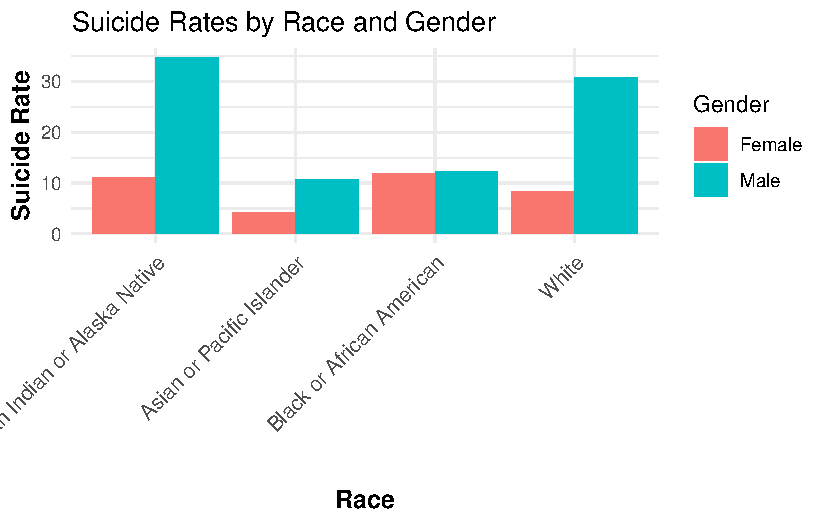
\includegraphics{Sec4_Team10_files/figure-pdf/unnamed-chunk-7-1.pdf}

}

\caption{Figure 1: Correlation Matrix}

\end{figure}%

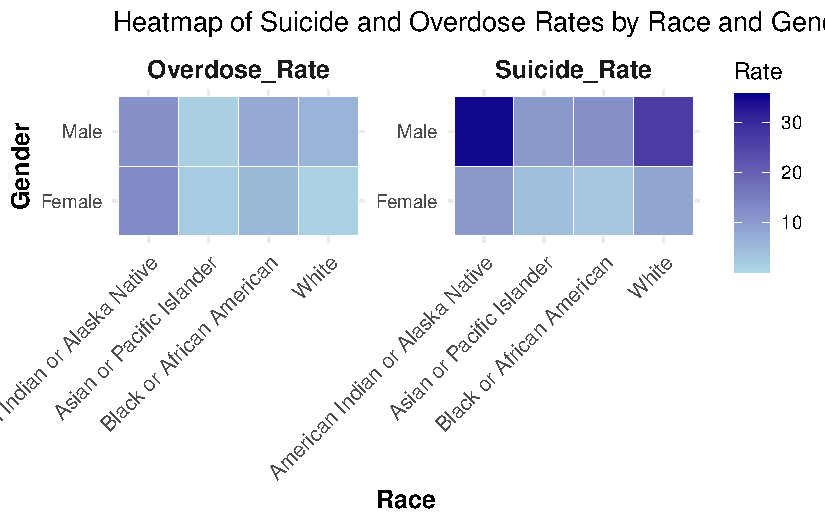
\includegraphics{Sec4_Team10_files/figure-pdf/unnamed-chunk-8-1.pdf}

This approach allowed me to analyze the data in detail, test the
hypotheses, and determine whether differences in suicide rates were
significantly influenced by ethnic, gender, or a combination of these
factors. The data, which were unequivocal and supported the rejection of
the null hypothesis, showed that there are significant differences
across gender, race, and their combinations. The alternative hypothesis
(H₁) states that there are significant differences in suicide rates,
suggesting that factors such as gender, race, or both influence the
rates displayed in the data. If at least one group shows a substantial
deviation, indicating a relationship between the observed suicide rates
and gender, race, or their interaction, the null hypothesis would be
rejected.

\begin{verbatim}
`summarise()` has grouped output by 'Race'. You can override using the
`.groups` argument.
\end{verbatim}

\begin{longtable}[]{@{}
  >{\raggedright\arraybackslash}p{(\columnwidth - 6\tabcolsep) * \real{0.3976}}
  >{\raggedright\arraybackslash}p{(\columnwidth - 6\tabcolsep) * \real{0.0843}}
  >{\raggedleft\arraybackslash}p{(\columnwidth - 6\tabcolsep) * \real{0.2530}}
  >{\raggedleft\arraybackslash}p{(\columnwidth - 6\tabcolsep) * \real{0.2651}}@{}}
\caption{Summary Table of Average Suicide and Overdose Rates by Race and
Gender}\tabularnewline
\toprule\noalign{}
\begin{minipage}[b]{\linewidth}\raggedright
Race
\end{minipage} & \begin{minipage}[b]{\linewidth}\raggedright
Gender
\end{minipage} & \begin{minipage}[b]{\linewidth}\raggedleft
Average Suicide Rate
\end{minipage} & \begin{minipage}[b]{\linewidth}\raggedleft
Average Overdose Rate
\end{minipage} \\
\midrule\noalign{}
\endfirsthead
\toprule\noalign{}
\begin{minipage}[b]{\linewidth}\raggedright
Race
\end{minipage} & \begin{minipage}[b]{\linewidth}\raggedright
Gender
\end{minipage} & \begin{minipage}[b]{\linewidth}\raggedleft
Average Suicide Rate
\end{minipage} & \begin{minipage}[b]{\linewidth}\raggedleft
Average Overdose Rate
\end{minipage} \\
\midrule\noalign{}
\endhead
\bottomrule\noalign{}
\endlastfoot
American Indian or Alaska Native & Female & 6.582609 & 5.7458333 \\
American Indian or Alaska Native & Male & 22.220652 & 7.9946341 \\
Asian or Pacific Islander & Female & 3.407500 & 0.7960784 \\
Asian or Pacific Islander & Male & 8.762500 & 1.3919118 \\
Black or African American & Female & 2.263830 & 2.5464029 \\
Black or African American & Male & 9.894444 & 5.8938433 \\
White & Female & 6.250000 & 4.2420290 \\
White & Male & 23.593478 & 8.0163043 \\
\end{longtable}

\subsection{Exploratory Data Analysis (EDA) for resesarch question
two}\label{exploratory-data-analysis-eda-for-resesarch-question-two}

The second research question, based on my topic, is: ``Is there a
significant difference in suicide rates between males and females across
racial groups?'' To answer this question, I analyzed the data in detail,
tested the hypotheses, and determined whether differences in suicide
rates were significantly influenced by ethnicity, gender, or their
combination. The approach used ensured a thorough examination of the
data, producing results that addressed the research question with
confidence. To begin, I claim the two hypotheses to guide the test. The
null hypothesis (H₀) assumed that there are no significant differences
in suicide rates across gender-race combinations, meaning that any
observed differences are purely random and there is no meanful.
Conversely, the alternative hypothesis (H₁) stated that there are
significant differences in suicide rates across these groups. This
hypothesis suggested that certain gender-race combinations might be more
vulnerable than others, indicating a relationship between the observed
suicide rates and the combination of gender and race. If at least one
group showed a substantial deviation, this would provide evidence to
reject the null hypothesis in favor of the alternative hypothesis.

The data analysis began with thorough cleaning and organization. I
started by assigning meaningful names to each group and removing
irrelevant or incomplete data that was not applicable to this research
question. Once cleaned, the dataset was categorized into three primary
components: gender (male and female), race (White, Black or African
American, American Indian or Alaska Native, and Asian or Pacific
Islander), and a gender-race combination variable. This categorization
was crucial as it allowed for a detailed examination of both the
independent effects of gender and race, as well as their interaction.
For example, while males overall might have higher suicide rates,
interaction analysis could reveal that certain racial groups within
males, such as American Indian or Alaska Native males, show
significantly higher rates than others. This organization ensured the
analysis was as thorough as possible and that no critical trends were
overlooked.And below was a my analyzed clean table.

Once the data was ready, I performed a Two-Way ANOVA (Analysis of
Variance) to determine whether the mean suicide rates differed
significantly by race, gender, and their interaction. The Two-Way ANOVA
is a statistical test designed to assess the effects of two independent
variables---gender and race in this case---on one dependent variable,
the suicide rates. The test addressed two primary questions: (1) whether
race and gender individually influence suicide rates (main effects), and
(2) whether the combination of gender and race creates unique patterns
that cannot be explained by their individual effects (interaction
effect). For instance, the main effect might show that males have higher
suicide rates than females, while the interaction effect could reveal
that White males or American Indian or Alaska Native males are
particularly vulnerable compared to other groups.

The results from the Two-Way ANOVA provided the first answer to my
research question by confirming that there were significant differences
in suicide rates between groups. However, while the ANOVA identified the
presence of significant differences, it could not pinpoint which
specific groups were different. To address this limitation, I used a
Tukey HSD (Honestly Significant Difference) post-hoc test, a statistical
method designed to compare the means of multiple groups while
controlling for Type I error (the risk of incorrectly identifying a
significant difference due to random chance). The Tukey HSD test builds
confidence intervals for each pairwise comparison between groups. If a
confidence interval does not include zero, it confirms that the
difference between the two groups is statistically significant. For
example, a confidence interval of {[}2.5, 7.0{]} for the difference in
suicide rates between males and females means the true difference lies
between 2.5 and 7.0, and since zero is not included, the difference is
substantial.

The Tukey HSD test results provided detailed insights. First, in terms
of gender, the findings showed that males consistently had significantly
higher suicide rates than females. This conclusion was strongly
supported by the confidence intervals, which were all positive and
excluded zero, indicating that the difference was unlikely to be random.
Next, the analysis turned to racial groups, revealing significant
patterns. For instance, Asian or Pacific Islanders had the lowest
overall suicide rates, while American Indian or Alaska Native
individuals had the highest rates of any racial group. These findings
suggested that race alone plays a substantial role in influencing
suicide rates.

Finally, when examining the combined effects of gender and race, the
interaction analysis revealed even more pronounced disparities. White
males and American Indian or Alaska Native males had the highest suicide
rates of any group, significantly higher than groups like Asian females
and Black females, which showed the lowest rates. The Tukey HSD test
validated these findings by showing that the confidence intervals for
these comparisons did not overlap zero, confirming their statistical
significance. In summary, the statistical analysis provided compelling
evidence that gender, race, and their combination significantly
influence suicide rates. The rejection of the null hypothesis (H₀) was
supported by both the ANOVA and Tukey HSD results. Across all racial
groups, males were consistently found to be at greater risk of suicide
compared to females. Additionally, racial disparities emerged, with
American Indian or Alaska Native individuals facing the highest risk
overall. When gender and race were combined, certain groups, such as
American Indian or Alaska Native males and White males, were identified
as particularly vulnerable. These findings underscore the importance of
analyzing gender and race together, as this approach revealed patterns
that would not have been apparent if the factors were examined
independently. By following this systematic methodology, I was able to
confidently answer the research question and uncover significant
relationships within the data.

\begin{verbatim}
[1] "Tukey HSD Test Results:"
\end{verbatim}

\begin{verbatim}
  Tukey multiple comparisons of means
    95% family-wise confidence level

Fit: aov(formula = Suicide_Rate ~ Gender * Race, data = cleaned_data)

$Gender
                diff      lwr      upr p adj
Male-Female 12.33521 12.20627 12.46415     0

$Race
                                                                  diff
Asian or Pacific Islander-American Indian or Alaska Native -8.31663043
Black or African American-American Indian or Alaska Native -8.27135642
White-American Indian or Alaska Native                      0.52010870
Black or African American-Asian or Pacific Islander         0.04527401
White-Asian or Pacific Islander                             8.83673913
White-Black or African American                             8.79146512
                                                                  lwr
Asian or Pacific Islander-American Indian or Alaska Native -8.5440960
Black or African American-American Indian or Alaska Native -8.5400499
White-American Indian or Alaska Native                      0.3007214
Black or African American-Asian or Pacific Islander        -0.2300549
White-Asian or Pacific Islander                             8.6092735
White-Black or African American                             8.5227717
                                                                  upr     p adj
Asian or Pacific Islander-American Indian or Alaska Native -8.0891649 0.0000000
Black or African American-American Indian or Alaska Native -8.0026630 0.0000000
White-American Indian or Alaska Native                      0.7394960 0.0000000
Black or African American-Asian or Pacific Islander         0.3206029 0.9746449
White-Asian or Pacific Islander                             9.0642047 0.0000000
White-Black or African American                             9.0601586 0.0000000

$`Gender:Race`
                                                                                     diff
Male:American Indian or Alaska Native-Female:American Indian or Alaska Native  15.6380435
Female:Asian or Pacific Islander-Female:American Indian or Alaska Native       -3.1751087
Male:Asian or Pacific Islander-Female:American Indian or Alaska Native          2.1798913
Female:Black or African American-Female:American Indian or Alaska Native       -4.3187789
Male:Black or African American-Female:American Indian or Alaska Native          3.3118357
Female:White-Female:American Indian or Alaska Native                           -0.3326087
Male:White-Female:American Indian or Alaska Native                             17.0108696
Female:Asian or Pacific Islander-Male:American Indian or Alaska Native        -18.8131522
Male:Asian or Pacific Islander-Male:American Indian or Alaska Native          -13.4581522
Female:Black or African American-Male:American Indian or Alaska Native        -19.9568224
Male:Black or African American-Male:American Indian or Alaska Native          -12.3262077
Female:White-Male:American Indian or Alaska Native                            -15.9706522
Male:White-Male:American Indian or Alaska Native                                1.3728261
Male:Asian or Pacific Islander-Female:Asian or Pacific Islander                 5.3550000
Female:Black or African American-Female:Asian or Pacific Islander              -1.1436702
Male:Black or African American-Female:Asian or Pacific Islander                 6.4869444
Female:White-Female:Asian or Pacific Islander                                   2.8425000
Male:White-Female:Asian or Pacific Islander                                    20.1859783
Female:Black or African American-Male:Asian or Pacific Islander                -6.4986702
Male:Black or African American-Male:Asian or Pacific Islander                   1.1319444
Female:White-Male:Asian or Pacific Islander                                    -2.5125000
Male:White-Male:Asian or Pacific Islander                                      14.8309783
Male:Black or African American-Female:Black or African American                 7.6306147
Female:White-Female:Black or African American                                   3.9861702
Male:White-Female:Black or African American                                    21.3296485
Female:White-Male:Black or African American                                    -3.6444444
Male:White-Male:Black or African American                                      13.6990338
Male:White-Female:White                                                        17.3434783
                                                                                      lwr
Male:American Indian or Alaska Native-Female:American Indian or Alaska Native  15.2719840
Female:Asian or Pacific Islander-Female:American Indian or Alaska Native       -3.5546472
Male:Asian or Pacific Islander-Female:American Indian or Alaska Native          1.8003528
Female:Black or African American-Female:American Indian or Alaska Native       -4.7639174
Male:Black or African American-Female:American Indian or Alaska Native          2.8601975
Female:White-Female:American Indian or Alaska Native                           -0.6986682
Male:White-Female:American Indian or Alaska Native                             16.6448101
Female:Asian or Pacific Islander-Male:American Indian or Alaska Native        -19.1926907
Male:Asian or Pacific Islander-Male:American Indian or Alaska Native          -13.8376907
Female:Black or African American-Male:American Indian or Alaska Native        -20.4019609
Male:Black or African American-Male:American Indian or Alaska Native          -12.7778459
Female:White-Male:American Indian or Alaska Native                            -16.3367117
Male:White-Male:American Indian or Alaska Native                                1.0067666
Male:Asian or Pacific Islander-Female:Asian or Pacific Islander                 4.9624449
Female:Black or African American-Female:Asian or Pacific Islander              -1.5999576
Male:Black or African American-Female:Asian or Pacific Islander                 6.0243139
Female:White-Female:Asian or Pacific Islander                                   2.4629615
Male:White-Female:Asian or Pacific Islander                                    19.8064397
Female:Black or African American-Male:Asian or Pacific Islander                -6.9549576
Male:Black or African American-Male:Asian or Pacific Islander                   0.6693139
Female:White-Male:Asian or Pacific Islander                                    -2.8920385
Male:White-Male:Asian or Pacific Islander                                      14.4514397
Male:Black or African American-Female:Black or African American                 7.1128060
Female:White-Female:Black or African American                                   3.5410317
Male:White-Female:Black or African American                                    20.8845100
Female:White-Male:Black or African American                                    -4.0960827
Male:White-Male:Black or African American                                      13.2473956
Male:White-Female:White                                                        16.9774188
                                                                                       upr
Male:American Indian or Alaska Native-Female:American Indian or Alaska Native  16.00410295
Female:Asian or Pacific Islander-Female:American Indian or Alaska Native       -2.79557015
Male:Asian or Pacific Islander-Female:American Indian or Alaska Native          2.55942985
Female:Black or African American-Female:American Indian or Alaska Native       -3.87364044
Male:Black or African American-Female:American Indian or Alaska Native          3.76347396
Female:White-Female:American Indian or Alaska Native                            0.03345078
Male:White-Female:American Indian or Alaska Native                             17.37692904
Female:Asian or Pacific Islander-Male:American Indian or Alaska Native        -18.43361363
Male:Asian or Pacific Islander-Male:American Indian or Alaska Native          -13.07861363
Female:Black or African American-Male:American Indian or Alaska Native        -19.51168392
Male:Black or African American-Male:American Indian or Alaska Native          -11.87456951
Female:White-Male:American Indian or Alaska Native                            -15.60459270
Male:White-Male:American Indian or Alaska Native                                1.73888556
Male:Asian or Pacific Islander-Female:Asian or Pacific Islander                 5.74755505
Female:Black or African American-Female:Asian or Pacific Islander              -0.68738278
Male:Black or African American-Female:Asian or Pacific Islander                 6.94957501
Female:White-Female:Asian or Pacific Islander                                   3.22203854
Male:White-Female:Asian or Pacific Islander                                    20.56551680
Female:Black or African American-Male:Asian or Pacific Islander                -6.04238278
Male:Black or African American-Male:Asian or Pacific Islander                   1.59457501
Female:White-Male:Asian or Pacific Islander                                    -2.13296146
Male:White-Male:Asian or Pacific Islander                                      15.21051680
Male:Black or African American-Female:Black or African American                 8.14842330
Female:White-Female:Black or African American                                   4.43130868
Male:White-Female:Black or African American                                    21.77478694
Female:White-Male:Black or African American                                    -3.19280623
Male:White-Male:Black or African American                                      14.15067203
Male:White-Female:White                                                        17.70953774
                                                                                 p adj
Male:American Indian or Alaska Native-Female:American Indian or Alaska Native 0.000000
Female:Asian or Pacific Islander-Female:American Indian or Alaska Native      0.000000
Male:Asian or Pacific Islander-Female:American Indian or Alaska Native        0.000000
Female:Black or African American-Female:American Indian or Alaska Native      0.000000
Male:Black or African American-Female:American Indian or Alaska Native        0.000000
Female:White-Female:American Indian or Alaska Native                          0.106855
Male:White-Female:American Indian or Alaska Native                            0.000000
Female:Asian or Pacific Islander-Male:American Indian or Alaska Native        0.000000
Male:Asian or Pacific Islander-Male:American Indian or Alaska Native          0.000000
Female:Black or African American-Male:American Indian or Alaska Native        0.000000
Male:Black or African American-Male:American Indian or Alaska Native          0.000000
Female:White-Male:American Indian or Alaska Native                            0.000000
Male:White-Male:American Indian or Alaska Native                              0.000000
Male:Asian or Pacific Islander-Female:Asian or Pacific Islander               0.000000
Female:Black or African American-Female:Asian or Pacific Islander             0.000000
Male:Black or African American-Female:Asian or Pacific Islander               0.000000
Female:White-Female:Asian or Pacific Islander                                 0.000000
Male:White-Female:Asian or Pacific Islander                                   0.000000
Female:Black or African American-Male:Asian or Pacific Islander               0.000000
Male:Black or African American-Male:Asian or Pacific Islander                 0.000000
Female:White-Male:Asian or Pacific Islander                                   0.000000
Male:White-Male:Asian or Pacific Islander                                     0.000000
Male:Black or African American-Female:Black or African American               0.000000
Female:White-Female:Black or African American                                 0.000000
Male:White-Female:Black or African American                                   0.000000
Female:White-Male:Black or African American                                   0.000000
Male:White-Male:Black or African American                                     0.000000
Male:White-Female:White                                                       0.000000
\end{verbatim}

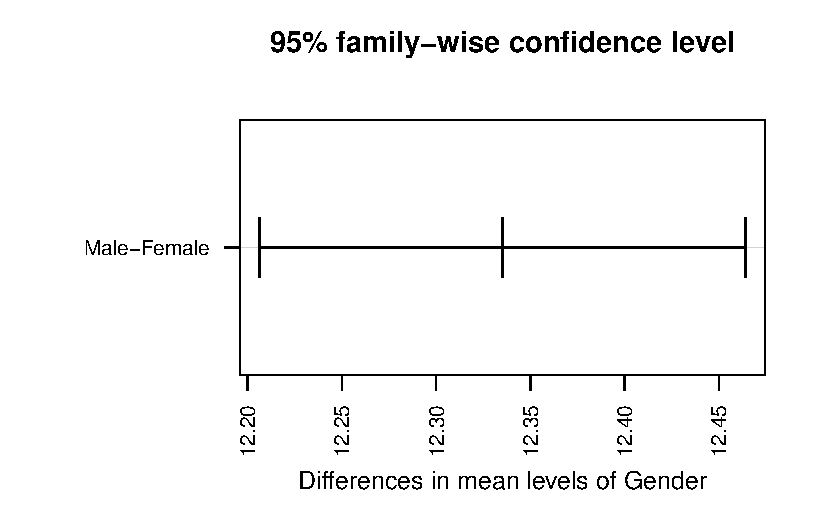
\includegraphics{Sec4_Team10_files/figure-pdf/unnamed-chunk-11-1.pdf}

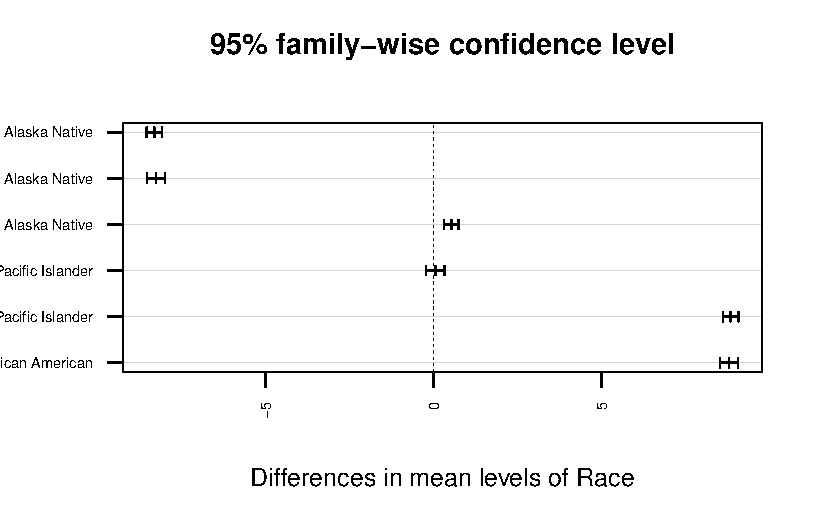
\includegraphics{Sec4_Team10_files/figure-pdf/unnamed-chunk-11-2.pdf}

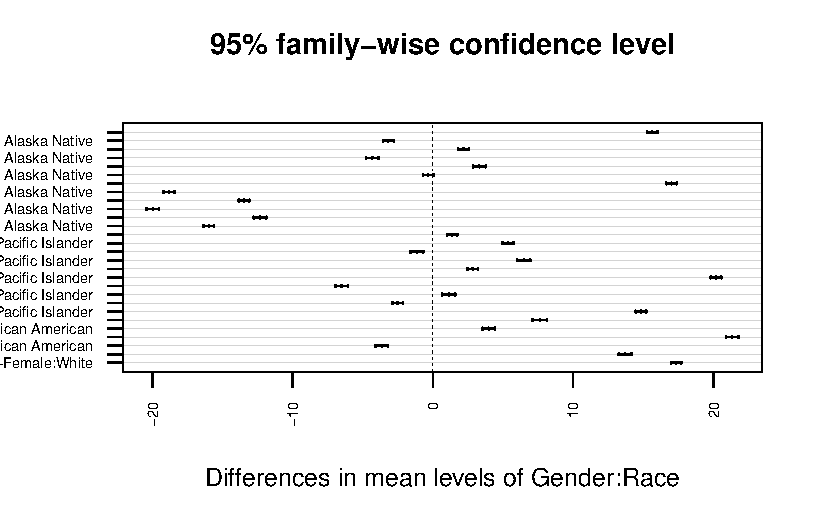
\includegraphics{Sec4_Team10_files/figure-pdf/unnamed-chunk-11-3.pdf}

\begin{Shaded}
\begin{Highlighting}[]
\CommentTok{\# This code will run, but the code and its output will be hidden.}
\FunctionTok{library}\NormalTok{(dplyr)}
\FunctionTok{library}\NormalTok{(tidyr)}
\NormalTok{suicide\_data }\OtherTok{\textless{}{-}} \FunctionTok{read.csv}\NormalTok{(}\StringTok{"C:/Users/hanzi/Downloads/Death\_rates\_for\_suicide\_\_by\_sex\_\_race\_\_Hispanic\_origin\_\_and\_age\_\_United\_States.csv"}\NormalTok{)}
\NormalTok{drug\_overdose\_data }\OtherTok{\textless{}{-}} \FunctionTok{read.csv}\NormalTok{(}\StringTok{"C:/Users/hanzi/Downloads/Drug\_overdose\_death\_rates\_\_by\_drug\_type\_\_sex\_\_age\_\_race\_\_and\_Hispanic\_origin\_\_United\_States.csv"}\NormalTok{)}
\CommentTok{\# Clean the suicide dataset}
\NormalTok{suicide\_clean }\OtherTok{\textless{}{-}}\NormalTok{ suicide\_data }\SpecialCharTok{\%\textgreater{}\%}
  \FunctionTok{mutate}\NormalTok{(}
    \AttributeTok{Gender =} \FunctionTok{case\_when}\NormalTok{(}
      \FunctionTok{grepl}\NormalTok{(}\StringTok{"Male"}\NormalTok{, STUB\_LABEL) }\SpecialCharTok{\textasciitilde{}} \StringTok{"Male"}\NormalTok{,}
      \FunctionTok{grepl}\NormalTok{(}\StringTok{"Female"}\NormalTok{, STUB\_LABEL) }\SpecialCharTok{\textasciitilde{}} \StringTok{"Female"}\NormalTok{,}
      \ConstantTok{TRUE} \SpecialCharTok{\textasciitilde{}} \StringTok{"All persons"}
\NormalTok{    ),}
    \AttributeTok{Race =} \FunctionTok{case\_when}\NormalTok{(}
      \FunctionTok{grepl}\NormalTok{(}\StringTok{"White"}\NormalTok{, STUB\_LABEL) }\SpecialCharTok{\textasciitilde{}} \StringTok{"White"}\NormalTok{,}
      \FunctionTok{grepl}\NormalTok{(}\StringTok{"Black or African American"}\NormalTok{, STUB\_LABEL) }\SpecialCharTok{\textasciitilde{}} \StringTok{"Black or African American"}\NormalTok{,}
      \FunctionTok{grepl}\NormalTok{(}\StringTok{"Asian or Pacific Islander"}\NormalTok{, STUB\_LABEL) }\SpecialCharTok{\textasciitilde{}} \StringTok{"Asian or Pacific Islander"}\NormalTok{,}
      \FunctionTok{grepl}\NormalTok{(}\StringTok{"American Indian or Alaska Native"}\NormalTok{, STUB\_LABEL) }\SpecialCharTok{\textasciitilde{}} \StringTok{"American Indian or Alaska Native"}\NormalTok{,}
      \ConstantTok{TRUE} \SpecialCharTok{\textasciitilde{}} \StringTok{"Unknown"}
\NormalTok{    )}
\NormalTok{  ) }\SpecialCharTok{\%\textgreater{}\%}
  \FunctionTok{select}\NormalTok{(}
\NormalTok{    Gender, }
\NormalTok{    Race,}
    \AttributeTok{Year =}\NormalTok{ YEAR,}
    \AttributeTok{Age\_Group =}\NormalTok{ AGE,}
    \AttributeTok{Suicide\_Rate =}\NormalTok{ ESTIMATE}
\NormalTok{  ) }\SpecialCharTok{\%\textgreater{}\%}
  \FunctionTok{filter}\NormalTok{(Gender }\SpecialCharTok{!=} \StringTok{"All persons"}\NormalTok{) }\CommentTok{\# Exclude general rows if needed}

\CommentTok{\# Clean the drug overdose dataset}
\NormalTok{drug\_overdose\_clean }\OtherTok{\textless{}{-}}\NormalTok{ drug\_overdose\_data }\SpecialCharTok{\%\textgreater{}\%}
  \FunctionTok{mutate}\NormalTok{(}
    \AttributeTok{Gender =} \FunctionTok{case\_when}\NormalTok{(}
      \FunctionTok{grepl}\NormalTok{(}\StringTok{"Male"}\NormalTok{, STUB\_LABEL) }\SpecialCharTok{\textasciitilde{}} \StringTok{"Male"}\NormalTok{,}
      \FunctionTok{grepl}\NormalTok{(}\StringTok{"Female"}\NormalTok{, STUB\_LABEL) }\SpecialCharTok{\textasciitilde{}} \StringTok{"Female"}\NormalTok{,}
      \ConstantTok{TRUE} \SpecialCharTok{\textasciitilde{}} \StringTok{"All persons"}
\NormalTok{    ),}
    \AttributeTok{Race =} \FunctionTok{case\_when}\NormalTok{(}
      \FunctionTok{grepl}\NormalTok{(}\StringTok{"White"}\NormalTok{, STUB\_LABEL) }\SpecialCharTok{\textasciitilde{}} \StringTok{"White"}\NormalTok{,}
      \FunctionTok{grepl}\NormalTok{(}\StringTok{"Black or African American"}\NormalTok{, STUB\_LABEL) }\SpecialCharTok{\textasciitilde{}} \StringTok{"Black or African American"}\NormalTok{,}
      \FunctionTok{grepl}\NormalTok{(}\StringTok{"Asian or Pacific Islander"}\NormalTok{, STUB\_LABEL) }\SpecialCharTok{\textasciitilde{}} \StringTok{"Asian or Pacific Islander"}\NormalTok{,}
      \FunctionTok{grepl}\NormalTok{(}\StringTok{"American Indian or Alaska Native"}\NormalTok{, STUB\_LABEL) }\SpecialCharTok{\textasciitilde{}} \StringTok{"American Indian or Alaska Native"}\NormalTok{,}
      \ConstantTok{TRUE} \SpecialCharTok{\textasciitilde{}} \StringTok{"Unknown"}
\NormalTok{    )}
\NormalTok{  ) }\SpecialCharTok{\%\textgreater{}\%}
  \FunctionTok{select}\NormalTok{(}
\NormalTok{    Gender,}
\NormalTok{    Race,}
    \AttributeTok{Year =}\NormalTok{ YEAR,}
    \AttributeTok{Age\_Group =}\NormalTok{ AGE,}
    \AttributeTok{Overdose\_Rate =}\NormalTok{ ESTIMATE}
\NormalTok{  ) }\SpecialCharTok{\%\textgreater{}\%}
  \FunctionTok{filter}\NormalTok{(Gender }\SpecialCharTok{!=} \StringTok{"All persons"}\NormalTok{) }\CommentTok{\# Exclude general rows if needed}
\CommentTok{\# Merge the two datasets}
\NormalTok{merged\_data }\OtherTok{\textless{}{-}} \FunctionTok{merge}\NormalTok{(}
\NormalTok{  suicide\_clean,}
\NormalTok{  drug\_overdose\_clean,}
  \AttributeTok{by =} \FunctionTok{c}\NormalTok{(}\StringTok{"Gender"}\NormalTok{, }\StringTok{"Race"}\NormalTok{, }\StringTok{"Year"}\NormalTok{, }\StringTok{"Age\_Group"}\NormalTok{),}
  \AttributeTok{all =} \ConstantTok{FALSE} 
\NormalTok{)}

\NormalTok{merged\_data }\OtherTok{\textless{}{-}}\NormalTok{ merged\_data }\SpecialCharTok{\%\textgreater{}\%}
  \FunctionTok{filter}\NormalTok{(Race }\SpecialCharTok{!=} \StringTok{"Unknown"}\NormalTok{) }\SpecialCharTok{\%\textgreater{}\%} \CommentTok{\# Remove rows with unknown race}
  \FunctionTok{select}\NormalTok{(}\SpecialCharTok{{-}}\NormalTok{Age\_Group, }\SpecialCharTok{{-}}\NormalTok{Year)     }\CommentTok{\# Drop the Age\_Group and Year columns entirely}

\FunctionTok{write.csv}\NormalTok{(merged\_data, }\StringTok{"Cleaned\_Combined\_Death\_Rates.csv"}\NormalTok{, }\AttributeTok{row.names =} \ConstantTok{FALSE}\NormalTok{)}
\FunctionTok{write.csv}\NormalTok{(}
\NormalTok{  merged\_data,}
  \StringTok{"C:/Users/hanzi/Downloads/Cleaned\_Combined\_Death\_Rates.csv"}\NormalTok{,}
  \AttributeTok{row.names =} \ConstantTok{FALSE}
\NormalTok{)}
\DocumentationTok{\#\# Image 1 for Question 1}
\FunctionTok{library}\NormalTok{(ggplot2)}
\CommentTok{\# Bar chart: Death rates by gender and race}
\FunctionTok{ggplot}\NormalTok{(}\AttributeTok{data =}\NormalTok{ merged\_data, }\FunctionTok{aes}\NormalTok{(}\AttributeTok{x =}\NormalTok{ Race, }\AttributeTok{y =}\NormalTok{ Suicide\_Rate, }\AttributeTok{fill =}\NormalTok{ Gender)) }\SpecialCharTok{+}
  \FunctionTok{geom\_bar}\NormalTok{(}\AttributeTok{stat =} \StringTok{"identity"}\NormalTok{, }\AttributeTok{position =} \StringTok{"dodge"}\NormalTok{) }\SpecialCharTok{+}
  \FunctionTok{theme\_minimal}\NormalTok{() }\SpecialCharTok{+}
  \FunctionTok{theme}\NormalTok{(}
    \AttributeTok{axis.text.x =} \FunctionTok{element\_text}\NormalTok{(}\AttributeTok{angle =} \DecValTok{45}\NormalTok{, }\AttributeTok{hjust =} \DecValTok{1}\NormalTok{, }\AttributeTok{size =} \DecValTok{10}\NormalTok{),}
    \AttributeTok{axis.title.x =} \FunctionTok{element\_text}\NormalTok{(}\AttributeTok{size =} \DecValTok{12}\NormalTok{, }\AttributeTok{face =} \StringTok{"bold"}\NormalTok{),}
    \AttributeTok{axis.title.y =} \FunctionTok{element\_text}\NormalTok{(}\AttributeTok{size =} \DecValTok{12}\NormalTok{, }\AttributeTok{face =} \StringTok{"bold"}\NormalTok{)}
\NormalTok{  ) }\SpecialCharTok{+}
  \FunctionTok{labs}\NormalTok{(}
    \AttributeTok{title =} \StringTok{"Suicide Rates by Race and Gender"}\NormalTok{,}
    \AttributeTok{x =} \StringTok{"Race"}\NormalTok{,}
    \AttributeTok{y =} \StringTok{"Suicide Rate"}\NormalTok{,}
    \AttributeTok{fill =} \StringTok{"Gender"}
\NormalTok{  )}
\DocumentationTok{\#\# Image 2 for Question 1}
\CommentTok{\# Load required library}
\FunctionTok{library}\NormalTok{(tidyr)}

\CommentTok{\# Transform data to long format}
\NormalTok{merged\_data\_long }\OtherTok{\textless{}{-}}\NormalTok{ merged\_data }\SpecialCharTok{\%\textgreater{}\%}
  \FunctionTok{pivot\_longer}\NormalTok{(}\AttributeTok{cols =} \FunctionTok{c}\NormalTok{(Suicide\_Rate, Overdose\_Rate), }
               \AttributeTok{names\_to =} \StringTok{"Variable"}\NormalTok{, }
               \AttributeTok{values\_to =} \StringTok{"Rate"}\NormalTok{)}

\CommentTok{\# Heatmap: Combined rates by race and gender}
\FunctionTok{library}\NormalTok{(ggplot2)}

\FunctionTok{ggplot}\NormalTok{(}\AttributeTok{data =}\NormalTok{ merged\_data\_long, }\FunctionTok{aes}\NormalTok{(}\AttributeTok{x =}\NormalTok{ Race, }\AttributeTok{y =}\NormalTok{ Gender, }\AttributeTok{fill =}\NormalTok{ Rate)) }\SpecialCharTok{+}
  \FunctionTok{geom\_tile}\NormalTok{(}\AttributeTok{color =} \StringTok{"white"}\NormalTok{) }\SpecialCharTok{+}
  \FunctionTok{facet\_wrap}\NormalTok{(}\SpecialCharTok{\textasciitilde{}}\NormalTok{ Variable, }\AttributeTok{scales =} \StringTok{"free"}\NormalTok{, }\AttributeTok{ncol =} \DecValTok{2}\NormalTok{) }\SpecialCharTok{+} \CommentTok{\# Adjust facets}
  \FunctionTok{scale\_fill\_gradient}\NormalTok{(}\AttributeTok{low =} \StringTok{"lightblue"}\NormalTok{, }\AttributeTok{high =} \StringTok{"darkblue"}\NormalTok{, }\AttributeTok{name =} \StringTok{"Rate"}\NormalTok{) }\SpecialCharTok{+}
  \FunctionTok{theme\_minimal}\NormalTok{() }\SpecialCharTok{+}
  \FunctionTok{theme}\NormalTok{(}
    \AttributeTok{axis.text.x =} \FunctionTok{element\_text}\NormalTok{(}\AttributeTok{angle =} \DecValTok{45}\NormalTok{, }\AttributeTok{hjust =} \DecValTok{1}\NormalTok{, }\AttributeTok{size =} \DecValTok{10}\NormalTok{), }\CommentTok{\# Rotate and space x{-}axis labels}
    \AttributeTok{axis.title.x =} \FunctionTok{element\_text}\NormalTok{(}\AttributeTok{size =} \DecValTok{12}\NormalTok{, }\AttributeTok{face =} \StringTok{"bold"}\NormalTok{),}
    \AttributeTok{axis.title.y =} \FunctionTok{element\_text}\NormalTok{(}\AttributeTok{size =} \DecValTok{12}\NormalTok{, }\AttributeTok{face =} \StringTok{"bold"}\NormalTok{),}
    \AttributeTok{strip.text =} \FunctionTok{element\_text}\NormalTok{(}\AttributeTok{size =} \DecValTok{12}\NormalTok{, }\AttributeTok{face =} \StringTok{"bold"}\NormalTok{) }\CommentTok{\# For facet titles}
\NormalTok{  ) }\SpecialCharTok{+}
  \FunctionTok{labs}\NormalTok{(}
    \AttributeTok{title =} \StringTok{"Heatmap of Suicide and Overdose Rates by Race and Gender"}\NormalTok{,}
    \AttributeTok{x =} \StringTok{"Race"}\NormalTok{,}
    \AttributeTok{y =} \StringTok{"Gender"}
\NormalTok{  )}
\DocumentationTok{\#\# Image 3 for Question 1}
\CommentTok{\# Summarize the data by Race and Gender}
\NormalTok{summary\_table }\OtherTok{\textless{}{-}}\NormalTok{ merged\_data }\SpecialCharTok{\%\textgreater{}\%}
  \FunctionTok{group\_by}\NormalTok{(Race, Gender) }\SpecialCharTok{\%\textgreater{}\%}
  \FunctionTok{summarise}\NormalTok{(}
    \AttributeTok{Avg\_Suicide\_Rate =} \FunctionTok{mean}\NormalTok{(Suicide\_Rate, }\AttributeTok{na.rm =} \ConstantTok{TRUE}\NormalTok{),}
    \AttributeTok{Avg\_Overdose\_Rate =} \FunctionTok{mean}\NormalTok{(Overdose\_Rate, }\AttributeTok{na.rm =} \ConstantTok{TRUE}\NormalTok{)}
\NormalTok{  )}

\CommentTok{\# Display the summary table}
\FunctionTok{library}\NormalTok{(knitr)}
\FunctionTok{kable}\NormalTok{(summary\_table, }
      \AttributeTok{col.names =} \FunctionTok{c}\NormalTok{(}\StringTok{"Race"}\NormalTok{, }\StringTok{"Gender"}\NormalTok{, }\StringTok{"Average Suicide Rate"}\NormalTok{, }\StringTok{"Average Overdose Rate"}\NormalTok{),}
      \AttributeTok{caption =} \StringTok{"Summary Table of Average Suicide and Overdose Rates by Race and Gender"}\NormalTok{)}
\CommentTok{\# Step 1: Load the dataset}
\NormalTok{data }\OtherTok{\textless{}{-}} \FunctionTok{read.csv}\NormalTok{(}\StringTok{"Cleaned\_Combined\_Death\_Rates.csv"}\NormalTok{)}

\CommentTok{\# Step 2: Clean the data}
\CommentTok{\# Select relevant columns and remove rows with missing values}
\NormalTok{cleaned\_data }\OtherTok{\textless{}{-}}\NormalTok{ data }\SpecialCharTok{\%\textgreater{}\%}
  \FunctionTok{select}\NormalTok{(Gender, Race, Suicide\_Rate) }\SpecialCharTok{\%\textgreater{}\%}
  \FunctionTok{na.omit}\NormalTok{()}

\CommentTok{\# Step 3: Perform Two{-}Way ANOVA}
\CommentTok{\# Test for differences in suicide rates between gender and racial groups}
\NormalTok{anova\_model }\OtherTok{\textless{}{-}} \FunctionTok{aov}\NormalTok{(Suicide\_Rate }\SpecialCharTok{\textasciitilde{}}\NormalTok{ Gender }\SpecialCharTok{*}\NormalTok{ Race, }\AttributeTok{data =}\NormalTok{ cleaned\_data)}

\CommentTok{\# Step 5: Perform Post{-}hoc Tukey HSD test}
\NormalTok{tukey\_results }\OtherTok{\textless{}{-}} \FunctionTok{TukeyHSD}\NormalTok{(anova\_model)}
\FunctionTok{print}\NormalTok{(}\StringTok{"Tukey HSD Test Results:"}\NormalTok{)}
\FunctionTok{print}\NormalTok{(tukey\_results)}

\CommentTok{\# Step 6: Adjust graphical parameters for better margins and readability}
\FunctionTok{par}\NormalTok{(}\AttributeTok{mar =} \FunctionTok{c}\NormalTok{(}\DecValTok{5}\NormalTok{, }\DecValTok{4}\NormalTok{, }\DecValTok{4}\NormalTok{, }\DecValTok{2}\NormalTok{) }\SpecialCharTok{+} \FloatTok{0.1}\NormalTok{)}
\FunctionTok{par}\NormalTok{(}\AttributeTok{cex.axis =} \FloatTok{0.6}\NormalTok{)        }\CommentTok{\# Reduce axis text size}
\FunctionTok{par}\NormalTok{(}\AttributeTok{las =} \DecValTok{2}\NormalTok{)               }\CommentTok{\# Rotate axis labels}

\CommentTok{\# Step 7: Plot Tukey HSD results}
\FunctionTok{plot}\NormalTok{(tukey\_results)}
\end{Highlighting}
\end{Shaded}




\end{document}
